\UseRawInputEncoding
\documentclass[runningheads]{llncs}
%\sloppy


\usepackage{xcolor}
\usepackage{listings}
\usepackage{inconsolata}
\usepackage{relsize}
%\usepackage{amsmath,amssymb,array}
\usepackage{mathpartir}
\usepackage{graphicx}
\usepackage{xspace}
\usepackage[colorlinks=true]{hyperref}
\usepackage{caption}

\newcommand{\Section}[1]{\vspace{-0ex}\section{#1}}
\newcommand{\SubSection}[1]{\vspace{-0ex}\subsection{#1}}
\newcommand{\Paragraph}[1]{\vspace{-1.0ex}\subsubsection{#1}} % lncs

\newcommand{\TODO}[2]{%
  \noindent\textcolor{gray}{%
      {\scriptsize\textbf{TODO(#1)}: #2}
  }
}

\setlength{\belowcaptionskip}{-1ex}
\setlength{\textfloatsep}{0.2ex}
\newenvironment{Figure}{
  \begin{figure}[tb]
} {
  \end{figure}
}

\newcommand{\MVP}[0]{\textsf{MVP}\xspace}
\newcommand{\solidity}[0]{\textsf{Solidity}\xspace}
\newcommand{\kay}[0]{\textsf{K}\xspace}
\newcommand{\fstar}[0]{\textsf{f*}\xspace}



% Source Transformation

\newcommand{\transform}[0]{\Large{$\leadsto$}}


%%%% Code

\usepackage[charter]{mathdesign}
%\def\rmdefault{bch}
%\def\ttdefault{blg}

\lstdefinestyle{MoveStyle}{
  basicstyle=\ttfamily,
  keywordstyle=\color{black}, % don't bold keywords which is the default
  escapechar=@, % use to embed LaTeX into code
  breaklines=true,
}


\lstdefinelanguage{Move}{
  morekeywords={
    abort,
    aborts_if,
    acquires,
    address,
    as,
    assert,
    assume,
    borrow_global,
    borrow_global_mut,
    break,
    const,
    continue,
    copy,
    copyable,
    define,
    drop,
    else,
    ensures,
    exists,
    false,
    forall,
    friend,
    fun,
    global,
    has,
    havoc,
    if,
    include,
    invariant,
    key,
    let,
    loop,
    modifies,
    module,
    move,
    move_from,
    move_to,
    mut,
    native,
    num,
    old,
    onabort,
    pragma,
    public,
    requires,
    resource,
    return,
    schema,
    script,
    signer,
    spec,
    store,
    struct,
    true,
    u8,
    u64,
    u128,
    update,
    use,
    with,
    where,
    while},
  sensitive=true,
  morecomment=[l]{//},
  morecomment=[s]{/*}{*/},
}

% This allows us to use |<move code>| for inline code.
\lstMakeShortInline[language=Move,style=MoveStyle]|


% This defines a new environment for Move code.
\lstnewenvironment{Move}{
  \lstset{
    language=Move,
    style=MoveStyle,
    basicstyle=\relsize{-1}\ttfamily,
    keywordstyle=\color{blue},
  }
}{
}

% This defines a new environment for Move code in a box, without line numbers.
\lstnewenvironment{MoveBox}{
  \lstset{
    language=Move,
    style=MoveStyle,
    basicstyle=\relsize{-1}\ttfamily,
    keywordstyle=\color{blue},
    %numbers=left,
    %numberstyle=\scriptsize\color{gray},
    %frame=single,
  }
}{
}

% This defines a new environment for Move code in a box, with line numbers.
\lstnewenvironment{MoveBoxNumbered}{
  \lstset{
    language=Move,
    style=MoveStyle,
    basicstyle=\relsize{-1}\ttfamily,
    keywordstyle=\color{blue},
    numbers=left,
    numberstyle=\scriptsize\color{gray},
    %frame=single,
  }
}{
}

% This defines a new environment for diagnostics as produced by the prover.
\lstnewenvironment{MoveDiag}{
  \lstset{
    style=MoveStyle,
    basicstyle=\relsize{-2}\ttfamily,
  }
}{
}




%%% Local Variables:
%%% mode: latex
%%% TeX-master: "main"
%%% End:


%\overfullrule=1mm


\begin{document}


\author{
  David Dill\inst{1} \and Wolfgang Grieskamp\inst{1} \and \\ Junkil
  Park\inst{1} \and Shaz Qadeer\inst{1} \and Meng Xu\inst{1}
  \and Emma Zhong\inst{1}
}

\institute{Novi Research, Facebook}
\authorrunning{D. Dill, W. Grieskamp et. al.}

\title{Fast and Reliable Formal Verification of Smart Contracts with the Move Prover}

\maketitle
\begin{abstract}
  The Move Prover (\MVP) is a formal verifier for smart contracts
  written in the Move programming language. \MVP has an expressive
  specification language, and is fast and reliable enough that it can
  be run routinely by developers and in integration testing in a few
  minutes. Besides the simplicity of smart contracts and the Move
  language, three transformations are responsible for the practicality
  of \MVP: (1) an alias-free memory model, (2) fine-grained invariant
  checking, and (3) monomorphization.  The entirety of the Move code for
  the Diem blockchain has been extensively specified and can be
  completely verified by \MVP in a few minutes. Changes in the Diem
  framework must be successfully verified before being integrated into
  the open source repository on GitHub.
  \keywords{Smart contracts \and
    formal verification \and Move language \and Diem blockchain}
\end{abstract}


\Section{Introduction}

The Move Prover (\MVP) is a formal verification tool for smart contracts that
intends to be used routinely during code development.  The verification finishes
fast and predictably, making the experience of running \MVP similar to the
experience of running compilers, linters, type checkers, and other development
tools.  Building a fast verifier is non-trivial, and in this paper, we would
like to share the most important engineering and architectural decisions that
have made this possible.

One factor that makes verification easier is applying it to smart contracts.
Smart contracts are easier to verify than conventional software for at least
three reasons: 1) they are small in code size, 2) they execute in a
well-defined, isolated environment, and 3) their computations are typically
sequential, deterministic, and have minimal interactions with the environment
(e.g., no explicit I/O operations).  At the same time, formal verification is
more appealing to the advocates for smart contracts becaues of the large
financial and regulatory risks that smart contracts may entail if misbehaved, as
evidenced by large losses that have occurred
already~\cite{CONTRACT_VERIFICATION,hacks-on-smart-contracts,hacks-on-compound}.

The other crucial factor to the success of \MVP is a tight coupling with the
\emph{Move} programming language~\cite{MOVE_LANG}.  Move is developed as part of
the Diem blockchain~\cite{DIEM} and is designed to be used with formal
verification from day one.  Move is currently co-evolving with \MVP.  The
language supports specifying pre-, post-, and aborts conditions of functions, as
well as invariants over data structures and over the content of the global
persistent memory (i.e., the state of the blockchain).  One feature that makes
verification harder is that universal and existential quantification can be used
freely in specifications.

Despite this specification richness, \MVP is capable of verifying the full Move
implementation of the Diem blockchain (called the Diem
framework~\cite{DIEM_FRAMEWORK}) in a few minutes.  The framework provides
functionality for managing accounts and their interactions, including multiple
currencies, account roles, and rules for transactions.  It consists of about
8,800 lines of Move code and 6,500 lines of specifications (including comments
for both), which shows that the framework is extensively specified.  More
importantly, \emph{verification is fully automated and runs continuously with
  unit and integration tests}, which we consider a testament to the practicality
of the approach.  Running the prover in integration tests requires more than
speed: it requires reliability, because tests that work sometimes and fail or
time out other times are unacceptable in that context.

\MVP is a substantial and evolving piece of software that has been tuned and
optimized in many ways.  As a result, it is not easy to define exactly what
implementation decisions lead to fast and reliable performance.  However, we can
at least identify three major ideas that resulted in dramatic improvements in
speed and reliability since the description of an early prototype of
\MVP~\cite{MOVE_PROVER}.  The rest of this paper focuses on these three core
ideas:
\begin{itemize}
\item an \emph{alias-free memory model} based on Move's semantics, which are
  similar to the Rust programming language;
\item \emph{fine-grained invariant checking}, which ensures that invariants hold
  at every state, except when developer explicitly suspends them; and
\item monomorphization, which instantiates type parameters in Move's generic
  structures, functions, and specification properties.
\end{itemize}
The combined effect of all these improvements transformed a tool that worked,
but often exhibited frustrating, sometimes random~\cite{BUTTERFLY}, timeouts on
complex and especially on erroneous specifications, to a tool that almost always
completes in less than 30 seconds.  In addition, there have been many other
improvements, including a more expressive specification language, reducing false
positives, and error reporting.

The remainder of the paper first introduces the Move language and how \MVP is
used with it, then discusses the design of \MVP and the three main optimizations
above.  There is also an appendix that describes injection of function
specifications.

%%% Local Variables:
%%% mode: latex
%%% TeX-master: "main"
%%% End:


\Section{Move and the Prover}

Move was developed for the Diem blockchain \cite{DIEM}, but its design is not
specific to blockchains.  A Move execution consists of a sequence of updates
evolving a \emph{global persistent memory state}, which we just call the
\emph{(global) memory}.  Updates are executed in a \emph{transactional} style.

The global memory is organized as a collection of resources, described by Move
structures (data types). A resource in memory is indexed by a pair of a type
(possibly instantiated) and an address (for example the address of a user
account). For instance, the expression |exists<Coin<USD>>(addr)| will be true if
there is a value of type |Coin<USD>| stored at |addr|. As seen in this example,
Move uses type generics, and working with generic functions and types is rather
idiomatic for Move.  Notice that account addresses are not just arbitrary values
but have a specific role in Move's programming methodology related to access
control via the builtin type of \emph{signers}, as will be discussed later.

A Move application consists of a set of \emph{transaction scripts}. Each of
those script defines a Move function with input parameters but no output
parameters.  This function updates the global memory, including emitting
events. The execution of this function can fail via a well-defined abort
mechanism, in which case the memory stays unmodified. An environment emits a
sequence of calls to such scripts, thereby evolving the memory.

% A transaction script is written in Move as an imperative function which can read
% and write the global memory. Move uses a specific style of
% imperative programming based on \emph{borrow semantics} \cite{BORROW_SEM}, as
% popularized in the programming language Rust \cite{RUST,RUST_TYPES}. For the
% verification problem borrow semantics is very important.  While allowing
% references into structured data, those are guaranteed to be safe by the
% \emph{borrow checker} \cite{BORROW_CHECKER}, which is run during bytecode
% loading time, and which verification can assume. Furthermore, the notorious hard
% verification problem of aliasing of references in the presence of mutation is
% eliminated.  Mutation always starts from a root location either in global memory
% or on the execution stack, and while a tree starting from this root is mutated,
% no other access can happen anywhere in the tree. Intuitively, borrow semantics
% allows to move a mutation 'cursor' down the tree, which follows linear typing
% discipline. Because of this property, mutable reference parameters to functions
% can be converted to input/output parameters, and verification of Move can avoid
% the traditionally hard problems caused by aliasing of mutable references.


\Paragraph{Programming in Move}

\begin{Figure}
\caption{\label{fig:AccountDef} Account Example Program}
\begin{MoveBox}
module Account {
  struct Account has key {
    balance: u64,
  }

  fun withdraw(account: address, amount: u64) acquires Account {
    let balance = &mut borrow_global_mut<Account>(account).balance;
    assert(*balance >= amount, Errors::limit_exceeded());
    *balance = *balance - amount;
  }

  fun deposit(account: address, amount: u64) acquires Account {
    let balance = &mut borrow_global_mut<Account>(account).balance;
    assert(*balance <= Limits::max_u64() - amount, Errors::limit_exceeded());
    *balance = *balance + amount;
  }

  public(script) fun transfer(from: &signer, to: address, amount: u64)
  acquires Account {
    assert(Signer::address_of(from) != to, Errors::invalid_argument());
    withdraw(Signer::address_of(from), amount);
    deposit(to, amount);
  }
}
\end{MoveBox}
\end{Figure}

\noindent In Move, one defines transactions via so-called \emph{script functions} which
take a set of parameters.  Those functions can call other functions. Script and
regular functions are encapsulated in \emph{modules}. Move modules are also the
place where structs are defined. An illustration of a Move contract is given in
Fig.~\ref{fig:AccountDef} (for a more complete description see the Move
Book~\cite{MOVE_LANG_DEF}). The example is a simple account which holds a
balance, defined in the script function |transfer|. Scripts get passed in so
called \emph{signers} which are tokens which represent an authorized account
address. The caller of the script -- an external program -- has ensured that the
owner of the signer account address has agreed to execute this script.  Notice
that in the code, the |assert| statement causes a Move transaction to abort
execution if the condition is not met.  Abortion can also happen implicitly; for
example, the expression |borrow_global_mut<T>(addr)| will abort if no resource
|T| exists at |addr|.


\Paragraph{Specifying in Move}

\begin{Figure}
\caption{\label{fig:AccountSpec} Account Example Specification}
\begin{MoveBox}
module Account {
  spec transfer {
    let from_addr = Signer::address_of(from);
    aborts_if from_addr == to;
    aborts_if bal(from_addr) < amount;
    aborts_if bal(to) + amount > Limits::max_u64();
    ensures bal(from_addr) == old(bal(from_addr)) - amount;
    ensures bal(to) == old(bal(to)) + amount;
  }

  spec fun bal(acc: address): u64 {
    global<Account>(acc).balance
  }

  invariant forall acc: address where exists<Account>(acc):
    bal(acc) >= AccountLimits::min_balance();

  invariant update forall acc: address where exists<Account>(acc):
    old(bal(acc)) - bal(acc) <= AccountLimits::max_decrease();
}
\end{MoveBox}
\end{Figure}

\noindent The specification language supports {\em Design By Contract}
\cite{DESIGN_BY_CONTRACT}. Developers can provide pre and post conditions for
functions, which include conditions over (mutable) parameters and global
memory. Developers can also provide invariants over data structures, as well as
the (state-dependent) content of the global memory. Universal and existential
quantification both over bounded domains (like the indices of a vector) as well
of unbounded domains (like all memory addresses, all integers, etc.)  are
supported. The latter makes the specification language very expressive, but also
renders the verification problem in theory undecidable (and in practice
dependent on heuristic decision procedures).

Fig.~\ref{fig:AccountSpec} illustrates the specification language by extending
the account example in Fig.~\ref{fig:AccountDef} (for the definition of the
specification language see \cite{MOVE_SPEC_LANG_DEF}). This adds the
specification of the |transfer| function, a helper function |bal| for use in
specs, and two global memory invariants. The first invariant states that a
balance can never drop underneath a certain minimum. The second invariant refers
to an update of global memory with pre and post state: the balance on an account
can never decrease in one step more than a certain amount.  Note that while the
Move programming language has only unsigned integers, the specification language
uses arbitrary precision signed integers, making it convenient to specify
something like |x + y <= limit|, without need to worry about overflow.

Specifications for the |withdraw| and |deposit| functions have been omitted in
this examples. \MVP supports omitting specs for non-recursive functions, in
which case they are treated as being inlined at caller site.

A discerning reader may have noted that the program in Fig.~\ref{fig:AccountDef}
does not actually satisfy the specification in Fig.~\ref{fig:AccountSpec}. This
will be discussed in the next section.

% The constructs we have seen so far are only a subset of the available features
% of the Move specification language. Notably, the language supports the following
% additional features:

% \begin{itemize}
% \item Function preconditions via the |requires|-clause.
% \item Data invariants for |struct| types, as a predicate over the field values.
% \item Means to abstract commonly used specification fragments in so-called
%   \emph{specification schemas} which can then be included in other specification
%   blocks.
% \end{itemize}

\Paragraph{Running the Prover}
\label{sec:RunningProver}

\MVP operates fully automated, quite similar to a type checker or linter, and is
expected to conclude in reasonable execution time, so it can be integrated in
the regular development workflow. Running \MVP on the |module Account| produces
multiple errors. The first is this one:

\begin{MoveDiag}
error: abort not covered by any of the `aborts_if` clauses
   -- account.move:24:3
   |
13 |       let balance = &mut borrow_global_mut<Account>(account).balance;
   |                          ----------------- abort happened here
   |
   =     at account.move:18: transfer
   =         from = signer{0x18be}
   =         to = 0x18bf
   =         amount = 147u8
   =     at ...
\end{MoveDiag}

\noindent \MVP detected that an implicit aborts condition is missing in the
specification of the |withdraw| function. It prints the context of the error, as
well as an \emph{execution trace} which lead to the error. Values of variable
assignments from the counterexample found by the SMT solver are printed together
with the execution trace. Logically, the counter example presents an instance of
assignments to variables such that program and specification disagree. In
general, \MVP attempts to produce diagnostics readable for Move developers
without the need of understanding any internals of the prover.

The next errors produced are about the memory invariants in
Fig.~\ref{fig:AccountSpec}. Both of them do not hold; we show only the first failure:

\begin{MoveDiag}
error: global memory invariant does not hold
   -- account.move:39:3
   |
39 |    invariant forall acc: address where exists<Account>(acc):
40 |      bal(acc) >= AccountLimits::min_balance();
   |
   =     at account.move:6: withdraw
   =         account = 0x0
   =         amount = 11u8
   =     at account.move:7: withdraw
   =         balance = &15u8
   =     at ...
\end{MoveDiag}

\noindent This happens because in the program in Fig.~\ref{fig:AccountDef}, we
did not made any attempt to respect the limits in |min_balance()| and
|max_decrease()|. We leave it open here (but covered it in
App.~\ref{sec:CorrectedAccount}) how to fix this problem, which requires
to add some more |assert| statements to the code and abort if the limits are not
met.

In reality, the programs and specifications \MVP deals with are significant larger than
in this example. For example, the conditions under which a transaction
in the Diem framework can abort typically has dozens of individual predicates,
stemming from other functions called by this transaction. Moreover, there are
hundreds of memory invariants specified, encoding access control and other
requirements for the Diem blockchain.

%%% Local Variables:
%%% mode: latex
%%% TeX-master: "main"
%%% End:

\Section{Move Prover Design}

\begin{Figure}
  \centering
  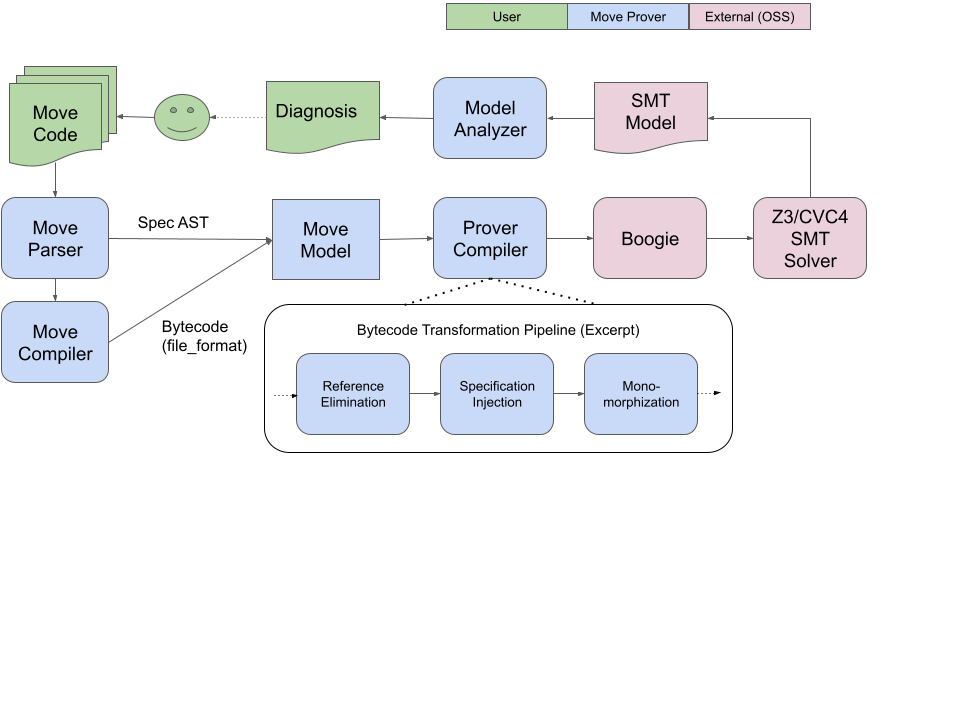
\includegraphics[trim=0 250 0 0, width=\textwidth]{arch.png}
  \caption{Move Prover Architecture}
  \label{fig:Arch}
\end{Figure}

The architecture of \MVP is illustrated in Fig.~\ref{fig:Arch}. Move code
(containing specifications) is given as input to the Move tool chain, which
produces two artifacts: the abstract syntax tree (AST) of the specifications,
and the generated bytecode.  The \emph{Move Model} merges both bytecode and
specifications, as well as other metdata from the original code, into a unique
object model which is input to the remaining tool chain.

The next phase is the actual \emph{Prover Compiler}, which is implemented as a
pipeline of bytecode transformations. Only an excerpt of the most important
transformations is shown (Reference Elimination, Specification Injection, and
Monomorphization). These transformations will be conceptually described in more
detail in subsequent sections. While they happen in reality on an extended
version of the bytecode, we will illustrate them on a higher level of
abstraction, as Move source level transformations.

The transformed bytecode is next compiled into the Boogie intermediate
verification language \cite{BOOGIE}. Boogie supports an imperative programming
model which is well suited for the encoding of the transformed Move code. Boogie
in turn can translate to multiple SMT solver backends, namely Z3 \cite{Z3} and
CVC5 \cite{CVC}; the default choice for the Move prover is currently Z3.

When the SMT solver produces a |sat| or |unknown| result (of the negation of the
verification condition Boogie generates), it produces a model witness. The Move
Prover attempts to translate this model back into a diagnostic which
a user can associate with the original Move code (as has been illustrated in
Sec.~\ref{sec:RunningProver}.) For example, execution traces leading to the
verification failure are shown, with assignments to variables used in this
trace, extracted from the model. Also the Move Model will be consulted to
retrieve the original source information and display it with the diagnosis.

Subsequently, we will focus on the major bytecode transformations.

\SubSection{Reference Elimination}
\label{sec:RefElim}

The Move language supports references to data stored in global memory and on the
stack. Those references can point to interior parts of the data. The reference
system is based on \emph{borrow semantics} \cite{BORROW_SEM} as it is also found
in the Rust programming language.  One can create (immutable) references |&x|
and mutable references |&mut x|, and derive new references by field selection
(|&mut x.f| and |&x.f|). The borrow semantics of Move provides the following
guarantees (ensured by the borrow checker~\cite{BORROW_CHECKER}):

\begin{itemize}
\item For any given location in global memory or on the stack, there can be
  either exactly one mutable reference, or $n$ immutable references. Hereby,
  it does not matter to what interior part of the data is referred to.
\item Dangling references to locations on the stack cannot exist; that is, the
  lifetime of references to data on the stack is restricted to the lifetime of the
  stack location.
\end{itemize}

\noindent These properties enable us to \emph{effectively eliminate} references from the Move
program, reducing the verification complexity significantly, as we do not need to
reason about sharing. It comes as no surprise that the same discipline of borrowing
which makes Move (and Rust) programs safer by design also makes verification simpler.

\Paragraph{Immutable References}

Since during the existance of an immutable reference no mutation on the
referenced data can occur, we can simply replace references by the referred
value.

An example of the applied transformation is shown below. We remove the reference
type constructor and all reference-taking operations from the code:

\begin{Move}
  fun select_f(s: &S): &T { &s.f } @\transform@ fun select_f(s: S): T { s.f }
\end{Move}


\noindent Notice that at Move execution time, immutable references serve
performance objectives (avoid copies); however, the symbolic reasoning engines
we use have a different representation of values, in which structure sharing is
common and copying is cheap.

\Paragraph{Mutable References}
\label{sec:RefElimMut}

Each mutation of a location |l| starts with an initial borrow for the whole data
stored in this location (in Move, |borrow_global_mut<T>(addr)| for global
memory, and |&mut x| for a local on the stack). Let's call the reference
resulting from such a borrow |r|. As long as this reference is alive, Move code
can either update its value (|*r = v|), or replace it with a sub-reference~%
(|r' = &mut r.f|). The mutation ends when |r| (or the derived |r'|) go out of
scope.  Because of the guarantees of the borrow semantics, during the mutation
of the data in |l| no other reference can exist into data in |l|.

The fact that |&mut| has exclusive access to the whole value in a location
allows to reduce mutable references to a \emph{read-update-write} cycle. One can
create a copy of the data in |l| and single-thread it to a sequence of
mutation steps which are represented as purely functional data updates.  Once
the last reference for the data in |l| goes out of scope, the updated value is
written back to |l|. This effectively turns an imperative program with references
into an imperative program which only has state updates on global memory or
variables on the stack, a class of programs which is known to have a significantly
simpler semantics. We illustrate the basics of this approach by an example:

\begin{Move}
  fun increment(x: &mut u64) { *x = *x + 1 }
  fun increment_field(s: &mut S) { increment(&mut s.f) }
  fun caller(): S { let s = S{f:0}; update(&mut s); s }
  @\transform@
  fun increment(x: u64): u64 { x + 1 }
  fun increment_field(s: S): S { s[f = increment(s.f)] }
  fun caller(): S { let s = S{f:0}; s = update(s); s }
\end{Move}

While the setup in this example covers a majority of the use cases in every day
Move code, there are more complex ones to consider, namely that the value of a
reference depends on runtime decisions. This is discussed in App.~\ref{sec:RefElimApx}.


\SubSection{Global Invariant Injection}
\label{sec:GlobalInvariants}

%% Dave comment: We discussed requiring update invariants to be transitive, but I don't think that's
%% a great idea after thinking about it more.  Too long to write here


% wrwg: Need to discuss that the commented model below is really what we want/have. It basically
% means that all invariants are always suspensable until transaction level, which is not what we
% are doing today (and their are reasons we don't want to).
%

\emph{Inductive} invariants are properties declared in Move modules that must
(by default) hold for the global memory at all times. Those invariants typically
quantify over addresses, as in~%
|invariant forall a: address: P(global<S>(a))|. See Fig.~\ref{fig:AccountSpec})
for examples. Based on Move's borrow semantics, inductive invariants don't need
to hold while memory is mutated; this is reflected by the reference elimination
described in Sec.~\ref{sec:RefElim}, and based on that the state of mutation is
not visible to anybody until it is written back to global memory.

\emph{Update} invariants are properties which relate two states.  Typically they
are enforced after an update of global memory, and are able to use the |old|
function to access the state before the update.

Verification of both kinds of global invariants can be \emph{suspended}. That
means, instead of being verified at the time a memory update happens, they are
verified at the call site of the function which updates memory. This is a
feature necessary to describe invariants over dependent parts of the global
memory which cannot be atomically updated.  Functions with external callers
(public or script functions) cannot suspend invariant verification, ensuring
that integrity of verification is preserved.


\Paragraph{Proof Methodology}

Inductive invariants are proved by induction over the evolution of the global
memory. The base case is that the invariant must hold in the empty state that
preceeds the genesis transaction.  For the induction step, we can assume that
the invariant holds at each verified function entry point for which it is not
suspended, and now must prove that it holds after program points which are
either direct updates of global memory, or calls to functions which suspend
invariants.

For update invariants, no soundness issue exist, as they just relate two
memories.  The pre-state is some memory captured before an update happens, and
the post state the current state. When an update invariant is suspended, it
should be designed to be transitive, such that its evaluation is not dependent
from the time of pre-state capture (e.g.~%
|invariant update [suspendable] version() >= old(version())| satisifies this
property).

%% Dave comment: I just noticed the next issue after writing the above paragraph.
%% If we only want to instrument instructions that change the types in invariant,
%% we need to make sure the invariant is valid when there are no changes.}
%% wrwg: only for suspended invariants, and then only if the update actually does
%% not happen in every path. However, the worst can happen is that if fails
%% verification, so seems no issue.
% We assume that an instruction that doesn't modify any of the types
% mentioned in an update invariant also does alter the validity of the invariant.
% Hence, an update invariant, regarded as a binary relation, must be reflexive.
% This property is not currently enforced by the prover.


% wrwg: This is discussed already
% Note that the induction proof
% allows the assumption of \textit{all} invariants at the beginning of each
% verified function to prove that an invariant holds after the function.  In
% practice, a subset of the available invariants are actually assumed on entry to
% a function. Some are not visible to the prover because they are specified
% outside of the cluster being verified, and others are excluded heuristically to
% reduce computational cost.


%% wrwg: we never tried this so don't know whether it is practical
% In some situations (such as blockchains), we would like
% users to be able to write transactions ``on-the-fly'' and submit
% them to the system, which does not allow time to run \MVP
% on individual transactions. The coarsest granularity we can
% practically achieve is to verify that each public and script function preserves
% inductive invariants.

\Paragraph{Modular Verification}

We wish to support open systems to which untrusted modules can be added to
without invalidating invariants that have already been proved. For each
invariant, there is a defined subset of Move modules (called a
\textit{cluster}). If the invariant is proved for the modules in the cluster, it
is guaranteed to hold in all other modules -- even those that were not yet
defined when the invariant was proved.  The cluster must contain every function
that can invalidate the invariant, and, in case of invariant suspension, all
callers of such a function.  Moreover, it must contain any function which calls
a friend function in a module for which the invariant is suspended. Importantly,
functions outside the cluster can never invalidate an invariant, so those
functions trivially preserve the invariant, so it is only necessary to verify
functions defined in the cluster.

\MVP verifies a given set of modules at a time (typically one).  The modules
being verified are called the \textit{target modules}, and the global invariants
to be verified are called \textit{target invariants}, which are all invariants
defined in the target modules. The cluster is then the smallest set as specified
above such that all target modules are contained.

\Paragraph{Basic Translation}

\begin{Figure}
  \caption{Basic Global Invariant Injection}
  \label{fig:GlobalInvariants}
  \centering
\begin{MoveBox}
  fun f(a: address) {
    let r = borrow_global_mut<S>(a);
    r.value = r.value + 1
  }
  invariant [I1] forall a: address: global<S>(a).value > 0;
  invariant [I2] update forall a: address:
      global<S>(a).value > old(global<S>(a).value);
  @\transform@
  fun f(a: address) {
    spec assume I1;
    Mvp::snapshot_state(I2_BEFORE);
    r = <increment mutation>;
    spec assert I1;
    spec assert I2[old = I2_BEFORE];
  }
\end{MoveBox}
\end{Figure}


%% Dave comment: Do we have standard terminology for the state
%%  variables upon which an invariant depends and that a function can
%%  access or modify? We should explain the concepts and terminology
%%  earlier and use them consistently throughout.
%%  wrwg: yes we do: "global memory", "memory update", "memory type"
%%    its defined in the move.tex but perhaps not consistently used

%%  wrwg: this is all already described below. Perhaps we should improve it
%%    instead of double writing
% The injection of assumes and asserts of global invariants into functions
% requires knowing whether a function reads or modifies memory that is mentioned
% in the invariant.  Without generic type parameters, this is a relatively simple
% analysis. First, the prover collects the set of memory types mentioned in the
% invariant.  For choosing the invariants to assume on entry to a function, \MVP
% collects all the types that are read or modified by the function or indirectly
% by functions that it calls, and intersects this set with the set of types in the
% invariant.  For choosing the invariants to assert, \MVP collects types that are
% modified by the function or by an individual instruction or function call and
% intersects that set with the set of types in the invariant.

We first look at injection of global invariants in the absence of memory and
functions with type parameters. Fig.~\ref{fig:GlobalInvariants} contains an
example for the supported invariant types and their injection into code. The
first invariant, |I1|, is an inductive invariant. It is assumed on function
entry, and asserted after the state update. The second, |I2|, is an update
invariant, which relates pre and post states. For this a state snapshot is
stored under some label |I2_BEFORE|, which is then used in an assertion.

Global invariant injection is optimized by knowledge of the prover, obtained by
static analysis, about accessed and modified memory.  Let |accessed(f)| be the
memory accessed by a function, and |modified(f)| the memory be modified. Let
|accessed(I)| by an invariant (including transitively by all functions it
calls).

\begin{itemize}
\item Inject |assume I| at entry to |f| \emph{if} |accessed(f)| has overlap with
  |accessed(I)|.
\item At every point in |f| where a memory location |M| is updated, or where a
  return from a function |f'| happens s.t. |M in modifies(f')| and for
  which |I| is suspended, inject |assert I| after the point \emph{if}~%
  |M in accessed(I)|. Also, if |I| is an update invariant, before the update or
  call inject a memory snapshot save.
\end{itemize}

\Paragraph{Genericity}

\begin{Figure}
  \caption{Global Invariant Injection and Genericity}
  \label{fig:Genericity}
  \centering
\begin{MoveBox}
  invariant [I1] global<S<u64>>(0).value > 1;
  invariant<T> [I2] global<S<T>>(0).value > 0;
  fun f(a: address) { borrow_global_mut<S<u8>>(0).value = 2 }
  fun g<R>(a: address) { borrow_global_mut<S<R>>(0).value = 3 }
  @\transform@
  fun f(a: address) {
    spec assume I2[T = u8];
    <<mutate>>
    spec assert I2[T = u8];
  }
  fun g<R>(a: address) {
    spec assume I1;
    spec assume I2[T = R];
    <<mutate>>
    spec assert I1;
    spec assert I2[T = R];
  }
\end{MoveBox}
\end{Figure}

Generic type parameters make the problem of determining whether a function can
modify an invariant more difficult.  For soundness, a property must hold for
every possible instantiation of type parameters.  So, rather than checking
whether some of the types mentioned in the invariant are equal to some of the
types accessed or modified by a function \MVP needs to discover whether there is
any possible instantiation of type parameters that might allow the instantiated
function to invalidate an instantiated invariant.  In other words, it needs to
know whether the each type in the invariant can be unified with a type accessed
or modified by the function.  Consider the example in
Fig.~\ref{fig:Genericity}. Invariant |I1| holds for a specific type
instantiation |S<u64>|, whereas |I2| is generic over all type instantiations for
|S<T>|.

The non-generic function |f| which works on the instantiation |S<u8>| will have
to inject the \emph{specialized} instance |I2[T = u8]|. The invariant |I1|,
however, does not apply for this function, because there is no overlap with
|S<u64>|.  In contrast, in the generic function |g| we have to inject both
invariants. Because this function works on arbitrary instances, it is also
relevant for the specific case of |S<u64>|.

In the general case, we are looking at a unification problem of the following
kind. Given the accessed memory of a function |f<R>| and an invariant |I<T>|, we
compute the pairwise unification of memory types. Those types are parameterized
over |R| resp. |T|, and successful unification will result in a substitution for
both. On successful unification, we include the invariant with |T| specialized
according to the substitution.

Notice that there are implications related to monomorphization coming from the
injection of global invariants; those are discussed in Sec.~\ref{sec:Mono}.


\SubSection{Monomorphization}
\label{sec:Mono}

Monomorphization is the process of removing all generic types from a Move
program by \emph{specializing the program for all relevant type instantiations}.
Like with genericity in most modern program languages, this is possible in Move
because the number of instantiations is statically known for a given program
fragment.

\Paragraph{Basic Monomorphization}

\begin{Figure}
\caption{Basic Monomorphization}
\label{fig:Mono}
\centering
\begin{MoveBox}
  struct S<T> { .. }
  fun f<T>(x: T) { g<S<T>>(S(x)) }
  fun g<S:key>(s: S) { move_to<S>(.., s) }
  @\transform@
  struct T{}
  struct S_T{ .. }
  fun f_T(x: T) { g_S_T(S_T(x)) }
  fun g_S_T(s: S_T) { move_to<S_T>(.., s) }
\end{MoveBox}
\end{Figure}

To verify a generic function, monomorphization skolemizes the type parameter
into a given type. It then, for all functions which are inlined, inserts their
code specializing it for the given type instantiation, including specialization
of all used types. Fig.~\ref{fig:Mono} sketches this approach.

The underlying conjecture is that if we verify |f_T|, we have also
verified it for all possible instantiations. However, this statement is
only correct for code which does not depend on runtime type information.

\Paragraph{Type Dependent Code}

The type of genericity Move provides does not allow for full type erasure as
often found in programming languages. That is because types are used to
\emph{index} global memory (e.g. |global<S<T>>(addr)| where |T| is a generic
type). Consider the following Move function:

\begin{Move}
  fun f<T>(..) { move_to<S<T>>(s, ..); move_to<S<u64>>(s, ..) }
\end{Move}

\noindent Depending on how |T| is instantiated, this function behaves
differently.  Specifically, if |T| is instantiated with |u64| the function will
always abort at the second |move_to|, since the target location is already
occupied.

The important property enabling monomorphization in the presence of type
dependent code is that one can identify the situation by looking at the memory
accessed by code and injected specifications. From this one can derive
\emph{additional instantiations of the function} which need to be verified. For
the example above, verifying both |f_T| and an instantiation |f_u64| will cover
all relevant cases of the function behavior. Notice that this treatment of type
dependent code is specific to the problem of verification, and cannot directly
be applied to execution.

The algorithm for computing the instances which require verification works as
follows. Let |f<T1,..,Tn>| be a verified target function which has all
specifications injected and inlined function calls expanded.
\begin{itemize}
\item Foreach memory |M in modifies(f)|, if there is a memory~%
  |M' in modifies(f)+accessed(f)| such that |M| and |M'| can unify via |T1,..,Tn|,
  collect an instaniation of the type parameters |Ti| from the resulting
  substitution. This instantiation may not assign values to all type parameters,
  and those unassigned parameters stay as is. For instance, |f<T1, T2>| might
  have a partial instantiation |f<T1, u8>|.
\item Once the set of all those partial instantiations is computed, it is
  extended by unifying the instantiations against each other. If |<t>| and
  |<t'>| are in the set, and they unify under the substitution |s|, then
  |<s(t)>| will also be part of the set.  For example, consider |f<T1, T2>|
  which modifies |M<T1>| and |R<T2>|, as well as accesses |M<u64>| and
  |R<u8>|. From this the instantiations |<u64, T2>| and |<T1, u8>| are computed,
  and the additional instantiation |<u64, u8>| will be added to the set.
\item If after computing and extending instantiations any type parameters
  remain, they are skolemized into a given type as described in the previous
  section.
\end{itemize}

To understand the correctness of this procedure, consider the following arguments:

\begin{itemize}
\item \emph{Direct interaction} Whenever a modified memory |M<t>| can influence
  the interpretation of |M<t'>|, a unifier must exist for the types |t| and |t'|,
  and an instantiation will be verified which covers the overlap of |t| and
  |t'|.
\item \emph{Indirect interaction} If there is an overlap between two types
  which influences whether another overlap is semantically relevant, the
  combination of both overlaps will be verified via the extension step.
\end{itemize}

Notice that even though it is not common in regular Move code to work with both
memory |S<T>| and, say, |S<u64>| in one function, there is a scenario where such
code is implicitly created by injection of global invariants. Consider the
example in Fig.~\ref{fig:Genericity}. The invariant |I1| which works on |S<u64>|
is injected into the function |g<R>| which works on |S<R>|. When monomorphizing
|g|, we need to verify an instance |g_u64| in order to ensure that |I1| holds.



%%% Local Variables:
%%% mode: latex
%%% TeX-master: "main"
%%% End:

\Section{Analysis}

\Paragraph{Reliability and Performance}

The three improvements described above resulted in a major qualitative
change in performance and reliability. In the version of \MVP released
in September 2020, correct examples verified fairly quickly and
reliably.  But that is because we needed speed and reliability, so we
disabled some properties that always timed out and others that timed
out unpredictably when there were small changes in the framework.  We
learned that incorrect programs or specifications would time out
predictably enough that it was a good bet that examples that timed out
were erroneous.  However, localizing the error to fix it was
\emph{very} hard, because debugging is based on a counterexample that
violates the property, and getting a counterexample requires
termination!

With each of the transformations described, we witnessed significant speedups
and, more importantly, reductions in timeouts.  Monomorphization was the last
feature implemented, and, with it, timeouts almost disappeared. Although this
was the most important improvement in practice, it is difficult to quantify
because there have been many changes in Diem framework, its specifications,
\MVP, and even the Move language over that time.

It is simpler (but less important) to quantify the changes in run time of \MVP
on one of our more challenging modules, the |DiemAccount| module, which is the
biggest module in the Diem framework. This module implements basic functionality
to create and maintain multiple types of accounts on the blockchain, as well as
manage their coin balances. It was called |LibraAccount| in release 1.0 of
\MVP. The table below lists the number of lines, functions, invariants,
conditions (requires, ensures, and aborts-if), as well as the verification
times:

{
\setlength{\tabcolsep}{6pt}
\vspace{2ex}
\begin{tabular*}{0.9\textwidth}{cccccc}
  \hline
  \hline
  Module & Lines & Functions & Invariants & Conditions & Timing \\
  \hline
  LibraAccount & 1975 & 72 & 10 & 113 & \textbf{9.131s} \\
  DiemAccount & 2554 & 64 & 32 & 171 & \textbf{6.290s} \\
  \hline
\end{tabular*}
\vspace{2ex}
}

\noindent Notice that |DiemAccount| has significantly grown in size compared to
the older version. Specifically, additional specifications have been
added. Moreover, in the original |LibraAccount|, some of the most complex
functions had to be disabled for verification because the old version of \MVP
would time out on them. In contrast, in |DiemAccount| and with the new version,
all functions are verified. Verification time has been improved by roughly 30\%,
in the presence of three times more global invariants, and 50\% more function
conditions.

We were able to observe similar improvements for the remaining of the 40 modules
of the Diem framework. All of the roughly half-dozen timeouts in verification in
the framework resolved after introduction of the transformations described in
this paper. Also, specifications which were introduced after the new
transformations did not introduce new timeouts.

%% A further improvement is that
%% often, in cases where specification and program disagree, a timeout occurred
%% which went away only after fixing the spec or the code, making debugging of such
%% verification failures rather hard. This problem also disappeared.


\Paragraph{Causes for the Improvements}

It's difficult to pin down and measure exactly why the three transformations
described improved performance and reliability so dramatically.  We have
explained some reasons in the subsections above: the alias-free memory model
reduced search through combinatorial sharing arrangments, and the fine-grained
invariant checking results in simpler formulas for the SMT solver.
%We believe that one reason is just that the translated SMT formulas are simpler.

We found that most timeouts in specifications stemmed from our liberal use of
quantifiers.  To disprove a property $P_0$ after assuming a list of properties,
$P_1, \ldots p_n$, the SMT solver must show that
$\neg P_0 \wedge P_1 \wedge \ldots \wedge P_n$ is satisfiable.  The search
usually involves instantiating universal quantifiers in $P_1, \ldots, P_n$.  The
SMT solver can do this endlessly, resulting in a timeout. Indeed, we often found
that proving a post-condition false would time out, because the SMT solver was
instantiating quantifiers to find a satisfying assignment of
$P_1 \wedge \ldots \wedge P_n$.  Simpler formulas result in fewer intermediate
terms during solving, resulting in fewer opportunities to instantiate quantified
formulas.

We believe that one of the biggest impacts, specifically on
removing timeouts and improving predictability, is monomorphization. The
reason for this is that monomorphization allows a multi-sorted representation
of values in Boogie (and eventually the SMT solver). In contrast, before
monomorphization, we used a universal domain for values in order to represent
values in generic functions, roughly as follows:

\begin{Move}
  type Value = Num(int) | Address(int) | Struct(Vector<Value>) | ...
\end{Move}

\noindent This creates a large overhead for the SMT solver, as we need to
exhaustively inject type assumptions (e.g. that a |Value| is actually an
|Address|), and pack/unpack values. Consider a quantifier like~%
|forall a: address: P(x)| in Move. Before monomorphization, we have to represent
this in Boogie as~%
|forall a: Value: is#Address(a) => P(v#Address(a))|. This quantifier is
triggered where ever |is#Address(a)| is present, independent of the structure of
|P|. Over-triggering or inadequate triggering of quantifiers is one of the
suspected sources of timeouts, as also discussed in~\cite{BUTTERFLY}.

Moreover, before monomorphization, global memory was indexed in Boogie by an
address and a type instantiation. That is, for |struct R<T>| we would
have one Boogie array |[Type, int]Value|. With monomorphization, the type index
is eliminated, as we create different memory variables for each type
instantiation.  Quantification over memory content works now on a one-dimensional
instead of an n-dimensional Boogie array.

\Paragraph{Discussion and Related Work}

Many approaches have been applied to the verification of smart contracts; see
e.g. the
surveys~\cite{liu2019survey,CONTRACT_VERIFICATION}. \cite{CONTRACT_VERIFICATION}
refers to at least two dozen systems for smart contract verification. It
distinguishes between \emph{contract} and \emph{program} level approaches. Our
approach has aspects of both: we address program level properties via pre/post
conditions, and contract (``blockchain state'') level properties via global
invariants. To the best of our knowledge, among the existing approaches, the
Move ecosystem is the first one where contract programming and specification
language are fully integrated, and the language is designed from first
principles influenced by verification. Methodologically, Move and the Move
prover are thereby closer to systems like Dafny~\cite{DAFNY}, or the older
Spec\# system~\cite{SPECSHARP}, where instead of adding a specification approach
posterior to an existing language, it is part from the beginning. This allows us
not only to deliver a more consistent user experience, but also to make
verification technically easier by curating the programming language.
% as reflected in Move's absence of
% dynamic dispatching and the notorious re-entrance problem~\cite{REENTRANCE}, as
% well as the borrow semantics which enables optimizations like reference
% elimination (Sec.~\ref{sec:RefElim}).

% Other related works on the
% \solidity smart contract verification employ the theoretical foundations
% including the \kay framework \cite{kay} (e.g., \cite{kevm}), \fstar
% \cite{dm4all} (e.g., \cite{DBLP:conf/ccs/BhargavanDFGGKK16,post2018}), and proof
% assistants such as Coq \cite{coqref} (e.g., \cite{fspvme,fether}).

In contrast to other approaches that only focus on specific vulnerability
patterns~\cite{mythril,oyente,maian,securify}, \MVP offers a universal
specification language. To the best of our knowledge, no existing specification
approach for smart contracts based on inductive Hoare logic has similar
expressiveness. We support universal quantification over arbitrary memory
content, a suspension mechanism of invariants to allow non-atomic construction
of memory content, and generic invariants.  For comparison, the SMT Checker
build into \solidity \cite{solidity,solcverify,DBLP:conf/esop/HajduJ20}
does not support quantifiers, because it interprets programming language
constructs (requires and assert statements) as specifications and has no
dedicated specification language. While in Solidity one can simulate aspects of
global invariants using modifiers by attaching pre/post conditions, this is not
the same as our invariants, which are guaranteed to hold independent of whether
a user may or (accidentally) may not attach a modifier, and which are optimized
to be only evaluated as needed.

While the expressiveness of Move specifications comes with the price of
undecidability and the dependency from heuristics in SMT solvers, \MVP deals
with this by its elaborated translation to SMT logic, as described in this
paper. The result is a practical verification system that is fully integrated
into the Diem blockchain production process, running in continuous integration,
which is (to the best of our knowledge) a first in the industry.

The invididual techniques we described are novel each by
themselves. \emph{Reference elimination} relies on borrow semantics, similar as
in the Rust~\cite{rust} language.  We expect reference elimination to apply for
the safe subset of Rust, though some extra work would be needed to deal with
references aggregated by structs.  However, we are not aware of that something
similar has been attempted in existing Rust verification work
\cite{prusti,smack,nopanic,crust}. \emph{Global invariant injection} and the
approach to minimize the number of assumptions and assertions is not applied in
any existing verification approach we know of; however, we co-authored a while
ago a similar line of work for \emph{runtime checking} of invariants in
Spec\#~\cite{StateConstraintsPatent}, yet that work never left the conceptual
state. \emph{Monomorphization} is well known as a technique for compiling
languages like C++ or Rust, where it is called specialization; however, we are
not aware of it being generalized for modular verification of generic code where
full type erasure is not possible, as it is the case in Move.


\Paragraph{Future Work}

\MVP is conceived as a tool for achieving higher assurance systems, not as a bug
hunting tool. Having at least temporarily achieved satsifactory performance and
reliability, we are turning our attention to the question of the goal of higher
assurance, which raises several issues.  If we're striving for high assurance,
it would be great to be able to measure progress towards that goal.  Since
system requirements often stem from external business and regulatory needs,
lightweight processes for exposing those requirements so we know what needs to
be formally specified would be highly desirable.

As with many other systems, it is too hard to write high-quality specifications.
Our current specifications are more verbose than they need to be, and we are
working to require less detailed specifications, especially for individual
functions.  We could expand the usefulness of \MVP for programmers if we could
make it possible for them to derive value from simple reusable specifications.
Finally, software tools for assessing the consistency and completeness of formal
specifications would reduce the risk of missing bugs because of specification
errors.

However, as more complex smart contracts are written and as more people write
specifications, we expect that the inherent computational difficulty of solving
logic problems will reappear, and there will be more opportunities for improving
performance and reliability.  In addition to translation techniques, it will be
necessary to identify opportunities to improve SMT solvers for the particular
kinds of problems we generate.


%%% Local Variables:
%%% mode: latex
%%% TeX-master: "main"
%%% End:

\Section{Conclusion}

We described key aspects of the Move prover (\MVP), a tool for formal
verification of smart contracts written in the Move language. \MVP has been
successfully used to verify large parts of the Diem framework, and is used in
continuous integration in production. The specification language is expressive,
specifically by the powerful concept of global invariants.  We described three
key implementation techniques which (as confirmed by our benchmarks) contributed
to the scalability of \MVP. One of the main areas of our future research is to
improve specification productivity and reduce the effort of reading and writing
specs, as well as to continue to improve speed and predictability of verification.



%%% Local Variables:
%%% mode: latex
%%% TeX-master: "main"
%%% End:


\vspace{-0.5ex}
\Paragraph{Acknowledgements}

This work would not have been possible without the many contributions of the
Move platform team and collaborators.  We specifically like to thank Bob Wilson,
Clark Barrett, Dario Russi, Jack Moffitt, Mathieu Baudet, Runtian Zhou, Sam
Blackshear, Tim Zakian, Todd Nowacki, Victor Gao, and Kevin Cheang.

\bibliographystyle{splncs04}
\bibliography{biblio}

\appendix
\newpage
\Section{Injection of Function Specifications}

During function specification injection, Move specifications are reduced to basic
assume/assert statements added to the Move code.  Those statements represent
instructions to the solver backend about what propositions can be assumed and
which need to be asserted (verified) at a given program point.  In this appendix,
we cover how \emph{function specification conditions} are injected.

\SubSection{Pre- and Post conditions}

The injection of basic function specifications is illustrated in
Fig.~\ref{fig:RequiresEnsuresAbortsIf}.  An extension of the Move source
language is used to specify abort behavior. With~%
|fun f() { .. } onabort { conditions }| a Move function is defined where
|conditions| are assume or assert statements that are evaluated at every program
point the function aborts (either implicitly or with an |abort| statement). This
construct simplifies the presentation and corresponds to a per-function abort
block on bytecode level which is target of branching.

\begin{Figure}
  \caption{Requires, Ensures, and AbortsIf Injection}
  \label{fig:RequiresEnsuresAbortsIf}
  \centering
\begin{MoveBoxNumbered}
  fun f(x: u64, y: u64): u64 { x + y }
  spec f {
    requires x < y;
    aborts_if x + y > MAX_U64;
    ensures result == x + y;
  }
  fun g(x: u64): u64 { f(x, x + 1) }
  spec g {
    ensures result > x;
  }
  @\transform@
  fun f(x: u64, y: u64): u64 {
    spec assume x < y;
    let result = x + y;
    spec assert result == x + y;     // ensures of f
    spec assert                      // negated abort_if of f
      !(x + y > MAX_U64); @\label{line:aborts_holds_not}@
    result
  } onabort {
    spec assert                      // abort_if of f
      x + y > MAX_U64; @\label{line:aborts_holds}@
  }
  fun g(x: u64): u64 {
    spec assert x < x + 1;           // requires of f
@$\textrm{\it if inlined}$\label{line:inline}@
    let result = inline f(x, x + 1);
@$\textrm{\it elif opaque}$\label{line:opaque}@
    if (x + x + 1 > MAX_U64) abort;  // aborts_if of f
    spec assume result == x + x + 1; // ensures of f
@$\textrm{\it endif}$@
    spec assert result > x;          // ensures of g
    result
  }
\end{MoveBoxNumbered}
\end{Figure}

An aborts condition is translated into two different asserts: one where the
function aborts and the condition must hold (line~\ref{line:aborts_holds}), and
one where it returns and the condition must \emph{not} hold
(line~\ref{line:aborts_holds_not}). If there are multiple |aborts_if|, they are
or-ed. If there is no abort condition, no asserts are generated. This means
that once a user specifies aborts conditions, they must completely cover the
abort behavior of the code. (The prover also provides an option to relax this
behavior, where aborts conditions can be partial and are only enforced on
function return.)

For a function call site we distinguish two variants: the call is \emph{inlined}
(line~\ref{line:inline}) or it is \emph{opaque} (line~\ref{line:opaque}).  For
inlined calls, the function definition, with all injected assumptions and
assertions turned into assumptions (as those are considered proven) is
substituted. For opaque functions the specification conditions are inserted as
assumptions. Methodologically, opaque functions need precise specifications
relative to a particular objective, where as in the case of inlined functions
the code is still the source of truth and specifications can be partial or
omitted. However, inlining does not scale arbitrarily, and can be only used for
small function systems.

Notice we have not discussed the way how to deal with relating pre and post
states yet, which requires taking snapshots of state (e.g.~%
|ensures x == old(x) + 1|); the example in
Fig.~\ref{fig:RequiresEnsuresAbortsIf} does not need it. Snapshots of state
will be discussed for global update invariants in Sec.~\ref{sec:GlobalInvariants}.

\Paragraph{Modifies}

\begin{Figure}
  \caption{Modifies Injection}
  \label{fig:Modifies}
  \centering
\begin{MoveBoxNumbered}
  fun f(addr: address) { move_to<T>(addr, T{}) }
  spec f {
    pragma opaque;
    ensures exists<T>(addr);
    modifies global<T>(addr);
  }
  fun g() { f(0x1) }
  spec g {
    modifies global<T>(0x1); modifies global<T>(0x2);
  }
  @\transform@
  fun f(addr: address) {
    let can_modify_T = {addr};      // modifies of f
    spec assert addr in can_modify; // permission check @%
                                            \label{line:modifies_permission}@
    move_to<T>(addr, T{});
  }
  fun g() {
    let can_modify_T = {0x1, 0x2};  // modifies of g
    spec assert {0x1} <= can_modify_T; // permission check @%
                                            \label{line:modifies_call_permission}@
    spec havoc global<T>(0x1);      // havoc modified memory @%
                                            \label{line:modifies_havoc}@
    spec assume exists<T>(0x1);     // ensures of f
  }
\end{MoveBoxNumbered}
\end{Figure}


The |modifies| condition specifies that a function only changes specific memory.
It comes in the form |modifies global<T>(addr)|, and its injection is
illustrated in Fig.~\ref{fig:Modifies}.

A type check is used to ensure that if a function has one or more~%
|modifies| conditions all called functions which are \emph{opaque} have a matching
modifies declaration. This is important so we can relate the callees
memory modifications to that what is allowed at caller side.

At verification time, when an operation is performed which modifies memory, an
assertion is emitted that modification is allowed
(e.g. line~\ref{line:modifies_permission}). The permitted addresses derived from
the modifies clause are stored in a set |can_modify_T| generated by the
transformation. Instructions which modify memory are either primitives (like
|move_to| in the example) or function calls. If the function call is inlined,
modifies injection proceeds (conceptually) with the inlined body. For opaque
function calls, the static analysis has ensured that the target has a modifies
clause.  This clause is used to derive the modified memory, which must be a
subset of the modified memory of the caller
(line~\ref{line:modifies_call_permission}).

For opaque calls, we also need to \emph{havoc} the memory they modify
(line~\ref{line:modifies_havoc}), by which is meant assigning an unconstrained
value to it. If present, |ensures| from the called function, injected as
subsequent assumptions, are further constraining the modified memory.


\Paragraph{Emits}

\begin{Figure}
  \caption{Emits Injection}
  \label{fig:Emits}
  \centering
\begin{MoveBoxNumbered}
  use Std::Event;
  struct E has drop, store { m: u64 }
  fun f(h: &mut Event::EventHandle<E>, x: u64) {
    Event::emit_event(h, E{m:0}); @\label{line:emit_event}@
    if (x > 0) {
      Event::emit_event(h, E{m:x});
    }
  }
  spec f {
    emits E{m:0} to h; @\label{line:emits}@
    emits E{m:x} to h if x > 0; @\label{line:emits_if}@
  }
  @\transform@
  fun f(h: &mut Event::EventHandle<E>, x: u64) {
    es = Mvp::ExtendEventStore(es, h, E{m:0}); // emitting event @\label{line:extend_es}@
    if (x > 0) {
      es = Mvp::ExtendEventStore(es, h, E{m:x}); // emitting event
    }
    let actual_es = Mvp::subtract(es, old(es)); // events emitted by f @\label{line:actual_es}@
    let expected_es = Mvp::CondExtendEventStore( // specified events @\label{line:expected_es}@
      Mvp::ExtendEventStore(Mvp::EmptyEventStore, E{m:x}, h),
      E{m:x}, h, x>0);
    spec assert Mvp::includes(expected_es, actual_es); // spec completeness @\label{line:emits_completeness}@
    spec assert Mvp::includes(actual_es, expected_es); // spec relevance @\label{line:emits_relevance}@
  }
\end{MoveBoxNumbered}
\end{Figure}

The injection for the |emits| clause is illustrated in Fig.~\ref{fig:Emits}. The |emits| clause specifies the events that a function is expected to emit. It comes in the form |emits message to handle if condition| (e.g., line~\ref{line:emits_if}). The condition part (i.e., |if condition|) can be omitted if the event is expected to be emitted unconditionally (e.g., line~\ref{line:emits}).

The function call to |Event::emit_event| (e.g., line~\ref{line:emit_event}) is transformed into the statement to extend |es| with the event to emit (e.g., line~\ref{line:extend_es}). |es| is a global variable of type |EventStore| which is a map where the key is an event handle and the value is the event stream of the handle (modeled as a bag of messages).

In line~\ref{line:actual_es}, |actual_es| represents the portion of the EventStore that only comprises the events that the program (i.e., |f|) actually emits. In line~\ref{line:expected_es}, |expected_es| is constructed from the |emits| specification which contains all of the expected events specified by the |emits| clauses. Having these, two assertions using |Mvp::includes| (multiset inclusion relation per event handle) are injected. One asserts that |expected_es| includes |actual_es|, meaning that the function only emits the events that are expected (e.g., line~\ref{line:emits_completeness}). This would be violated if there is any event emitted by |f| that is not covered by some |emits| clause. Another asserts that |actual_es| includes |expected_es|, meaning that the function emits all of the events that are expected (e.g., line~\ref{line:emits_relevance}). This would be violated if |f| does not emit the expected event which a |emits| clause specifies.

We also handle opaque calls properly although it is not illustrated in Fig.~\ref{fig:Emits}. Suppose |f| is an opaque function, and another function |g| calls |f|. In the transformation of |g|, the event store |es| extends with the expected events of |f| (i.e., the events specified by the |emits| clauses of |f|) in a similar way to how |expected_es| is constructed in line~\ref{line:expected_es}.

\vspace{-2ex}
\SubSection{Data Invariants}

\begin{Figure}
  \caption{Data Invariant Injection}
  \label{fig:DataInvariants}
  \centering
\begin{MoveBoxNumbered}
  struct S { a: u64, b: u64 }
  spec S { invariant a < b }
  fun f(s: S): S {
    let r = &mut s;
    r.a = r.a + 1;
    r.b = r.b + 1;
    s
  }
  @\transform@
  fun f(s: S): S {
    spec assume s.a < s.b;      // assume invariant for s
    let r = Mvp::local(s, F_s); // begin mutation of s
    r = Mvp::set(r, Mvp::get(r)[a = Mvp::get(r).a + 1]);
    r = Mvp::set(r, Mvp::get(r)[b = Mvp::get(r).b + 1]);
    spec assert                 // invariant enforced
      Mvp::get(r).a < Mvp::get(r).b;
    s = Mvp::get(r);            // write back to s
    s
  }
\end{MoveBoxNumbered}
\end{Figure}

A data invariant specifies a constraint over a struct value. The value is
guaranteed to satisfy this constraint at any time. Thus, when a value is
constructed, the data invariant needs to be verified, and when it is consumed,
it can be assumed to hold.

In Move's reference semantics, construction of struct values is often done via a
sequence of mutations via mutable references. It is desirable that \emph{during}
such mutations, assertion of the data invariant is suspended. This allows to
state invariants which reference multiple fields, where the fields are updated
step-by-step.  Move's borrow semantics and concept of mutations provides a
natural way how to defer invariant evaluation: at the point a mutable reference
is released, mutation ends, and the data invariant can be enforced.  In other
specification formalisms, we would need a special language construct for
invariant suspension. Fig.~\ref{fig:DataInvariants} gives an example, and shows
how data invariants are reduced to assert/assume statements.

The implementation of data invariants hooks into the reference elimination
(Sec.~\ref{sec:RefElim}). As part of this the lifetime of references is
computed. Whenever a reference is released and the mutated value is written
back, we also enforce the data invariant. In addition, the data invariant is
enforced when a struct value is directly constructed.


%%% Local Variables:
%%% mode: latex
%%% TeX-master: "main"
%%% End:

\newpage
\Section{Corrected Account Example}
\label{sec:CorrectedAccount}

To fix the verification errors from the account example in  Fig.~\ref{fig:AccountDef}
and Fig.~\ref{fig:AccountSpec}, the following changes would need to be made:

\begin{MoveBox}
module Account {
  ...

  fun withdraw(account: address, amount: u64) acquires Account {
    assert(amount <= AccountLimits::max_decrease(), Errors::invalid_argument()); // MISSING
    let balance = &mut borrow_global_mut<Account>(account).balance;
    assert(*balance >= amount, Errors::limit_exceeded());
    assert(*balance - amount >= AccountLimits::min_balance(), Errors::invalid_argument()); // MISSING
    *balance = *balance - amount;
  }

  spec transfer {
    ...
    aborts_if !exists<Account>(from_addr); // MISSING
    aborts_if !exists<Account>(to); // MISSING
    aborts_if amount > AccountLimits::max_decrease(); // MISSING
    aborts_if bal(from_addr) - amount < AccountLimits::min_balance(); // MISSING
  }
}
\end{MoveBox}


%%% Local Variables:
%%% mode: latex
%%% TeX-master: "main"
%%% End:



\end{document}


%%% Local Variables:
%%% mode: latex
%%% TeX-master: t
%%% End:
